%%%%%%%%%%%%%%%%%%%%%%%%%%%%%%%%%%%%%%%%%%%%%%%%%%%%%%%%%%%%%%%%%%%%%%%%%%%%%%%%
%2345678901234567890123456789012345678901234567890123456789012345678901234567890
%        1         2         3         4         5         6         7         8

\documentclass[letterpaper, 10 pt, conference]{ieeeconf}  % Comment this line out
                                                          % if you need a4paper
%\documentclass[a4paper, 10pt, conference]{ieeeconf}      % Use this line for a4
                                                          % paper

%\IEEEoverridecommandlockouts                              % This command is only
                                                          % needed if you want to
                                                          % use the \thanks command
\overrideIEEEmargins
% See the \addtolength command later in the file to balance the column lengths
% on the last page of the document

% This is needed to prevent the style file preventing citations from linking to 
% the bibliography
\makeatletter
\let\NAT@parse\undefined
\makeatother

\usepackage[dvipsnames]{xcolor}

\newcommand*\linkcolours{ForestGreen}

\usepackage{times}
\usepackage{xcolor, soul}
\sethlcolor{yellow}
\usepackage{graphicx}
\usepackage{amssymb}
\usepackage{gensymb}
\usepackage{amsmath}
\usepackage{breakurl}
\def\UrlBreaks{\do\/\do-}
\usepackage{url,hyperref}
\hypersetup{
colorlinks,
linkcolor=\linkcolours,
citecolor=\linkcolours,
filecolor=\linkcolours,
urlcolor=\linkcolours}

\usepackage{algorithm}
\usepackage{algorithmic}

\usepackage[labelfont={bf},font=small]{caption}
\usepackage[none]{hyphenat}

\usepackage{mathtools, cuted}

\usepackage[noadjust, nobreak]{cite}
\def\citepunct{,\,} % Style file defaults to listing references separately

\usepackage{tabularx}
\usepackage{amsmath}

\usepackage{float}

\usepackage{pifont}% http://ctan.org/pkg/pifont
\newcommand{\cmark}{\ding{51}}%
\newcommand{\xmark}{\ding{55}}%

\newcommand*\diff{\mathop{}\!\mathrm{d}}
\newcommand*\Diff[1]{\mathop{}\!\mathrm{d^#1}}
\newcommand*\imgres{600}

\newcommand*\GitHubLoc{https://github.com/Jeffrey-Ede/ALRC}

\newcolumntype{Y}{>{\centering\arraybackslash}X}

%\usepackage{parskip}

\usepackage[]{placeins}

% \usepackage{epstopdf}
% \epstopdfDeclareGraphicsRule{.tif}{png}{.png}{convert #1 \OutputFile}
% \AppendGraphicsExtensions{.tif}

\newcommand\extraspace{3pt}

\usepackage{placeins}

\usepackage{tikz}
\newcommand*\circled[1]{\tikz[baseline=(char.base)]{
            \node[shape=circle,draw,inner sep=0.8pt] (char) {#1};}}
            
\usepackage[framemethod=tikz]{mdframed}

\usepackage{afterpage}

\usepackage{stfloats}

\usepackage{atbegshi}
\newcommand{\handlethispage}{}
\newcommand{\discardpagesfromhere}{\let\handlethispage\AtBeginShipoutDiscard}
\newcommand{\keeppagesfromhere}{\let\handlethispage\relax}
\AtBeginShipout{\handlethispage}

\usepackage{comment}

%\usepackage[1,2,3,5,6,7]{pagesel} %Discard page 4 as it is blank

% The following packages can be found on http:\\www.ctan.org
%\usepackage{graphics} % for pdf, bitmapped graphics files
%\usepackage{epsfig} % for postscript graphics files
%\usepackage{mathptmx} % assumes new font selection scheme installed
%\usepackage{times} % assumes new font selection scheme installed
%\usepackage{amsmath} % assumes amsmath package installed
%\usepackage{amssymb}  % assumes amsmath package installed

\title{\LARGE \bf
Clustering and Classification of ICS Sensor Data
}


\author{Caleb Huck, M. Rayhan Ahmed Mithu, Zishan Ahmed Onik%
}

\begin{document}


\maketitle
\thispagestyle{empty}
\pagestyle{empty}


%%%%%%%%%%%%%%%%%%%%%%%%%%%%%%%%%%%%%%%%%%%%%%%%%%%%%%%%%%%%%%%%%%%%%%%%%%%%%%%%
\begin{abstract}
Modern Industrial Control Systems (ICS) have not kept pace with the evolving security landscape in recent decades, leaving them vulnerable and open to attack. Developing robust security measures in this domain is tricky due to the nature of the systems themselves. ICSs often have highly variable requirements and specifications that result in much heterogeneity in the hardware. Often, these systems consists of low power/low resource edge devices that are not capable of the computation cost of robust modern cryptography algorithms. Therefore, it is advantageous to seek security solutions that put the burden on devices in the system that have the resources necessary to facilitate the security measures being employed. Many past works attempt to achieve this by applying data mining to network packets. There are several issues with this approach. We instead focus on sensor state data that could theoretically be obtained directly from a PLC's memory. For our project, we apply data mining techniques to a test dataset as a proof-of-concept that we can effectively model sensor state data. 
\end{abstract}

%%%%%%%%%%%%%%%%%%%%%%%%%%%%%%%%%%%%%%%%%%%%%%%%%%%%%%%%%%%%%%%%%%%%%%%%%%%%%%%%
\section{INTRODUCTION}
Industrial Control Systems (ICS) facilitate the operation and monitoring of various large-scale systems in many different domains such as manufacturing, smart grids, health care, water and waste control, nuclear plants, and oil and gas refining. These systems communicate with many remote nodes to perform various tasks for remote control and monitoring of operations. ICSs generally use a master/slave configuration where a master node (such as a PLC or RTU) communicates with a slave node (such as a sensor or actuator) via control messages \cite{igure2006security}.

Historically, these systems were isolated to a specific area of operation on a private network. There was no connection to the open internet, and therefore little motivation to develop protocols with built-in security measures. Hence, security took a back seat to performance and feature related considerations \cite{igure2006security}. However, as the demand for increased connectivity and interoperability increased, this dynamic evolved to what we see today. ICS systems are more connected than ever, and consequently, more vulnerable than ever. This is evident in data from \cite{byres2004myths} showing a drastic uptrend in ratio of inside threats to outside threats from 1982 to 2003. Prior to 2001, 69\% of all threats were classified as ``accidental" or ``Internal" (such as a disgruntled employee. However, between 2001 and 2003, 70\% of threats were external. This data presents a significant shift that has likely only continued to grow in magnitude since the study was conducted.

Due to the increase in connectivity and frequency of attacks on ICS systems in recent times, ICS security has become a major focus of research. Many of the devises deployed in ICS networks are simple, low power devices with limited capability. Hence, it is difficult and generally infeasible to simply port popular security solutions like cryptography over for use in ICS systems. Therefore, there is much motivation to develop novel security approaches that are robust, yet not too computation-intensive for low power devices to handle. 
One approach to this problem is to utilize machine learning to categorize system behavior for the purpose of intrusion detection. Many solutions exist that apply this method to network data \cite{ponomarev2015industrial, schuster2013towards, feng2017multi, terai2017cyber, hijazi2018deep}. The problem is that there often isn't enough information in the network packets to make a confident decision. Additionally, if the network is already compromised, packets may be spoofed to appear normal to the IDS system. For this reason, we have explored the viability of using machine learning techniques to identify edge nodes based on node status data that would be stored on a PLC. For this purpose, we have employed two types of data mining technique, namely, clustering and classification.


%%%%%%%%%%%%%%%%%%%%%%%%%%%%%%%%%%%%%%%%%%%%%%%%%%%%%%%%%%%%%%%%%%%%%%%%%%%%%%%%
\section{Research Questions}
\begin{itemize}
    \item Can we effectively use clustering techniques to determine how many types of nodes are in a given data set?
    \item Can we accurately classify ICS sensor data into groups representing the type of sensor that the data originated from?
    \item Which classification algorithm will yield the best results?
    \item Is performance an important metric?
\end{itemize}

%%%%%%%%%%%%%%%%%%%%%%%%%%%%%%%%%%%%%%%%%%%%%%%%%%%%%%%%%%%%%%%%%%%%%%%%%%%%%%%%
\section{Methodology}
Our methodology is divided into four sections. The first section deals with data set selection criteria and selection process. The second section will discuss the data preprocessing that was necessary. The third section will discuss our clustering algorithm and the validation methods we used. Finally, the fourth section will go into depth on the classification portion of our project.

\subsection{Data Set Selection}
Initially, we planned to use the ICS test bed in the HPC lab of Tennessee Tech to generate our own data set. Unfortunately, the timing didn't work for this to take place. So we began researching publicly available data sets that would suffice instead. As previously mentioned, most current studies focus on network data rather than data stored directly by the PLC. This limited our options in terms of available data sets that would meet our particular needs. We wanted a data set that contained data from at least three different types of sensors (although more would be better). We also wanted to have data collected over a long enough time interval so that we would have an adequate amount of data points to train our classifiers. Based on these criteria, we narrowed it down to 5 data sets:
\begin{enumerate}
    \item Power system dataset consisting of two power generators, and four IEDs that control four breakers. This dataset includes 37 event scenarios, some of which are attack events \cite{pan2015developing}.
    \item Labeled RTU telemetry streams taken from a gas pipeline system in Mississippi State University's Critical Infrastructure Protection Center. This dataset also contains examples of normal operating as well as data taken while the system was being attacked \cite{beaver2013evaluation}.
    \item Dataset containing data collected from two laboratory ICSs. One is a gas pipeline and the other is a water storage tank. This dataset also contains data with and without attacks present \cite{morris2011control}.
    \item Dataset developed from the previous gas pipeline dataset but with more randomness \cite{morris2015industrial}.
    \item Dataset taken from two coastal wind farms in Brazil containing four sensor types and data taken over the course of one year \cite{passos_sakagami_santos_haas_taves_2017}.
\end{enumerate}

Based on our criteria, we decided that dataset 5 was the best fit for our project. For our preliminary results, we thought it would be better to not include data from attack events, which all of the other datasets have. Additionally, dataset 5 meets our criteria of three or more sensor types and duration of data collection (each file contains more than 40,000 entries). Based on this, we determined that dataset 5 was the best choice.

\subsection{Data pre-processing}
The coastal wind farm data set was in NetCDF format. The NetCDF or Network Common Data Form is a abstraction for storing heterogeneous multidimensional data. NetCDF format is very popular with scientific community because NetCDF supports storage and retrieval of machine independent and self-describing data, which is very difficult to achieve with commonly used data format like CSV. However to simply our work and to focus on clustering we decided to convert the NetCDF dataset into CSV format.

The NetCDF dataset from coastal wind farm contains 43 variables from 32 wind turbines. A NetCDF variable is, in simplest a term an array of values of same type. A NetCDF variable has a dimension, a name and some meta-data describing the variable. A single NetCDF file can have multiple variable, with different data type, dimensions and attributes. In our case, each variable of the coastal wind farm dataset represented different measurements from the 32 turbines. But we were interested in only 4 of the variables namely, "Wind speed", "Rotor RPM", "Active Power", "ACT Position", because only these variables directly came from a some kind of sensors.

From the Single NetCDF file 32 separate CSV files were generated each corresponding a one of the 32 turbines.

Further processing was performed to improve the performance of clustering algorithms. The initial data with four sensors did not produce expected result. Each row in the dataset contained value for all the four sensors which resulted cluster being to close to each other with similar features. To create a much more clean and distinguishable dataset, it w s

a\begin{figure}[htb]
    \centering
    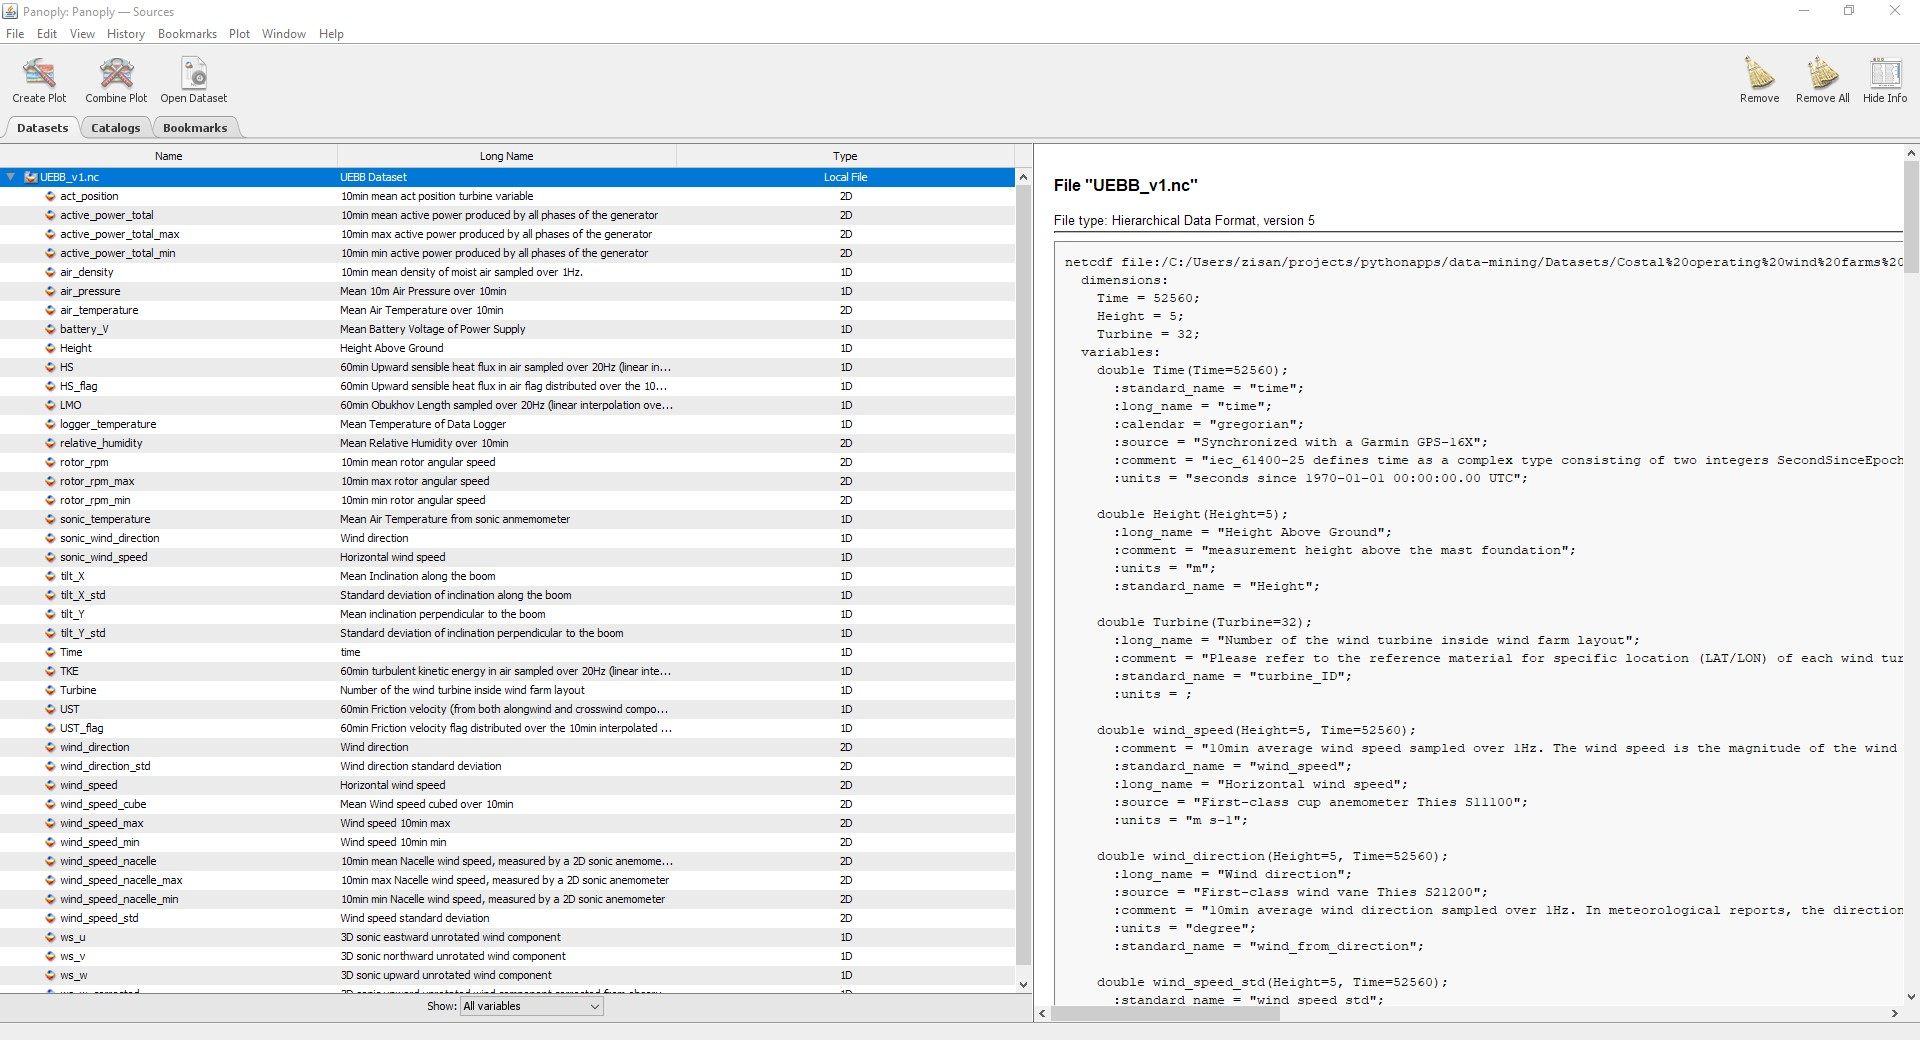
\includegraphics[width=10cm]{nc.jpg}
    \caption{Variables in The NetCDF Dataset}
\end{figure}


\subsection{Clustering}



\begin{figure}[htb]
    \centering
    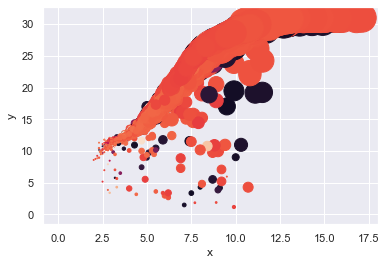
\includegraphics[scale=0.60]{cluster.png}
    \caption{Initial Clustering Results}
    \label{fig:init_cluster}
\end{figure}

\begin{figure}[htb]
    \centering
    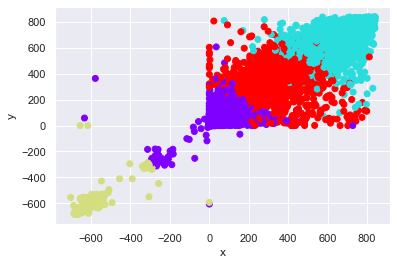
\includegraphics[scale=0.60]{cluster_update.png}
    \caption{Updated Clustering}
    \label{fig:updated_cluster}
\end{figure}


\subsection{Classification}
Classification is a form of supervised learning that essentially takes some input, and based on the input, predicts the category of the object. This is done in two phases. The first phase is the training phase, where a prediction model is built based on some dataset that is fed in to the algorithm. Once the model is constructed, it can be used to make individual predictions when it sees new data analogous to what it has observed. 
For our project, we have selected four common classification algorithms that we believed would yield positive results for our problem:

\textbf{Decision Trees}--- Decision trees are a type of prediction model that utilizes the tree data structure where each node in the tree contains several key components. Figure \ref{fig:DT_Subtree} shows a graphic example of a sub-tree with leaf nodes generated from our decision tree model using the graphviz package (the entire tree would be far too large to fit on a page). This tree is constructed using an algorithm during training. We used the sklearn package for python which uses a variation of the CART (Classicfication and Regression Trees) algorithm \cite{scikit-learn}. This prediction model works by traversing the tree starting at the root and working toward a leaf node (which represents a decision). The fist entry in the node is a conditional statement that determines which node will be explored next. The gini score is a measure of how ``pure" the node is \cite{ceballos_2020}. Essentially this is a measure of how many classes are represented at this node that where a score greater than zero indicates that some items belong to different samples. Conversely, if the gini score is zero, this means that only one class is represented and thus, a decision node has been reached. 

\begin{figure}[hbt]
    \centering
    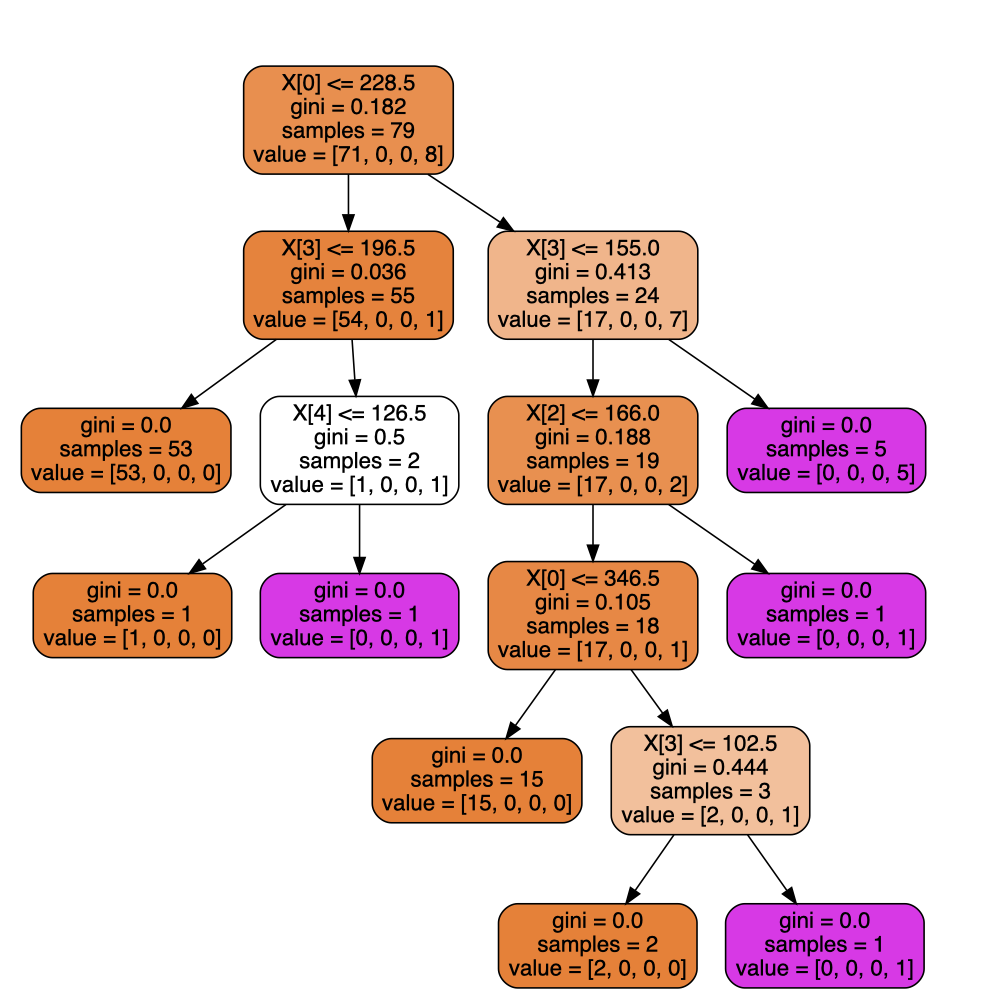
\includegraphics[scale=0.25]{DT_Tree_Graph.png}
    \caption{Decision Tree Subtree}
    \label{fig:DT_Subtree}
\end{figure}

\textbf{K-Nearest-Neighbor (KNN)}--- KNN is a technique that compares a feature set with every other feature set in the dataset to find the \textit{k} closest feature sets in terms of Euclidean distance. The formula for Euclidean distance between two points $X=(x_1, x_2,...,x_n)$ and $Y=(y_1, y_2,...,y_n)$ is defined as
\begin{equation}
d(X, Y)=\sqrt{\sum_{i=1}^{n} (x_i - y_i)^2}
\end{equation}
Once the \textit{k} nearest neighbors are found, the most common class represented by the neighbors is assigned to the unknown feature set. In practice, \textit{k} is an integer parameter that can be specified prior to classification. In our case, we determined the optimal value of \textit{k} experimentally by testing all odd values between 1 and $\sqrt{n}$ (where $n$ is the number of entries in the dataset). The reason we test only odd values is to prevent tied voting when the majority class among nearest neighbors is determined. The tested \textit{k} values are then graphed against the produced f-measure to determine the optimal value. Figure

\begin{figure}
    \centering
    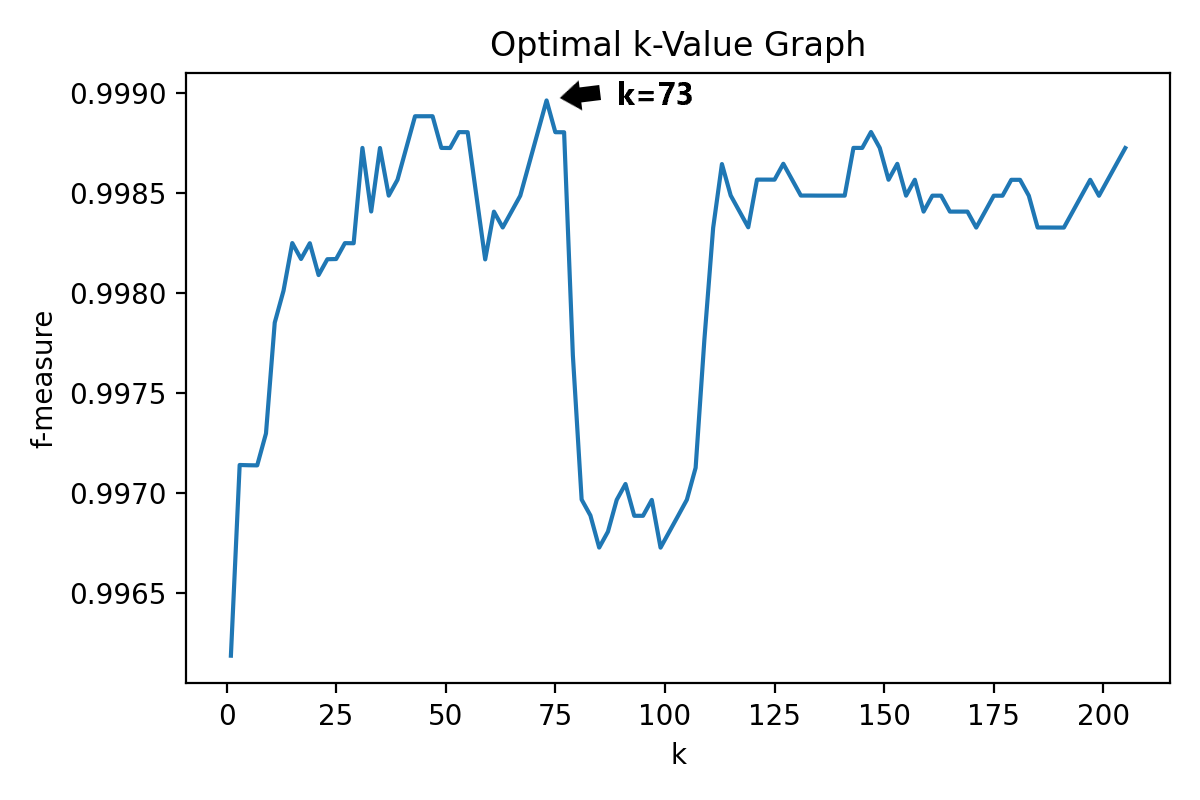
\includegraphics[scale=0.25]{k_vals_plot.png}
    \caption{Plot of \textit{k} values against F-measure}
    \label{fig:my_label}
\end{figure}

KNN is known as a lazy classifier since this computation is done at prediction time. In fact, KNN does not build a prediction model ahead of time at all. Rather, all samples must be stored in memory so that when an unknown sample is presented, the nearest neighbors can be calculated on demand. For this reason, KNN is generally faster than eager learners (learners that build models ahead of time) for training, but slower at predicting (especially if the training set is very large) \cite{phyu2009survey}. 

\textbf{Support Vector Machines (SVM)}--- This technique begins by uses a non-linear mapping of the training data to a higher dimension. The algorithm then searches for a ``linear optimal separating hyperplane". This is essentially a decision boundary that is used to choose between classes. SVM searches for what is known as the Maximum Marginal Hyperplane. If the dataset is linearly separable (i.e., it is possible to separate the data by a straight line or plane, depending on the number of dimensions), then there are an infinite number of possible hyperplanes that separate the data. The maximum marginal hyperplane is one that maximizes the distance between itself and the data that it separates as shown in figure \ref{fig:SVM_Hyperplane}. The idea is that this will maximize the probability that unseen data will fall on correct side of the hyperplane and thus be classified correctly \cite{han2011data}.  

\begin{figure}
    \centering
    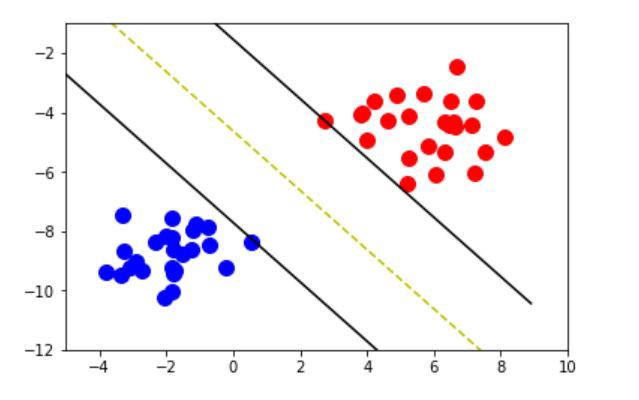
\includegraphics[scale=0.4]{SVM_Hyperplane.jpeg}
    \caption{SVM Hyperplane \cite{sanjeevi_mady_2018}}
    \label{fig:SVM_Hyperplane}
\end{figure}

\textbf{Na\"{i}ve Bayes}--- Na\"{i}ve Bayes is a type of Bayesian Network where certain assumptions are made in terms of the data attributes. Essentially, it is a statistical classification technique that relies on calculating probabilities among the training data using Bayes' theorem, which is a way to represent conditional probabilities. Bayes' theorem is defined as
\begin{equation}
    P(X|Y)=\dfrac{P(Y|X)P(X)}{P(Y)}
\end{equation}
Na\"{i}ve Bayes makes the assumption that all attributes are independent of each other. This allows for the extending of this relationship to multiple input variables by simply multiplying their probabilities together according to
\begin{equation}
    P(x|y_1, y_2,...,y_n)=\dfrac{P(y_1|x)P(y_2|x)...P(y_n|x)P(x)}{P(y_1)P(y_2)...P(y_n)}
\end{equation}
Given these relationships, the Na\"{i}ve Bayes classifier is able to calculate and store probabilities based on the training data to form a prediction model. When an unknown sample is fed to the prediction model, it will simply plug in the stored values for each probability of the attributes in the unknown sample and calculate the probability of the sample belonging to each class. The class with the highest calculated probability will then be assigned to the sample \cite{nikam2015comparative}.  


\section{Individual Contributions}
This section will describe the individual contributions of team members and how our project came together. As mentioned before, in the beginning stages of the project, we were waiting for the testbed in the HPC lab to become available so that we could collect our data. During this time, all of us were assigned the same task, which was to research datasets that we could use if the HPC testbed didn't work out. We spent time doing this together in person where we could discuss aspects of the datasets, as well as individually. After this initial collective task, individual tasks were assigned to each team member, which will be described below.

\textbf{Caleb Huck ---} after the first version of our clustering algorithm did not work as expected, I was assigned a task to write a script that would transpose sections of data so that they would line up correctly for the clustering algorithm. My next task was to take the code from the decision tree classifier and modify it to create the other three classifiers. I later added code to generate f-measure scores and the confusion matrices that we use to demonstrate our results in the Findings section below. I also modified the KNN classifier to find the optimal \textit{k} and graph the results. Lastly, I modified the decision tree classifier to include graphing functionality (graphviz) that allows us to see the generated tree.

\textbf{}


%%%%%%%%%%%%%%%%%%%%%%%%%%%%%%%%%%%%%%%%%%%%%%%%%%%%%%%%%%%%%%%%%%%%%%%%%%%%%%%%
\section{Findings}
The results from our experiments have been mostly very positive. However, unsupervised learning did not yield the best results. Our updated clustering (figure \ref{fig:updated_cluster}) shows much better results compared to the initial clusters in figure \ref{fig:init_cluster}. To validate our clustering, we used silhouette scores as well as Davies-Bouldin (DB) index scores for number of clusters ranging from 2-6. The scores are shown in table \ref{tab:cluster_scores}. For the DB index, a score closer to 0 indicates better separation in the clustering \cite{deycheck_dey_2019}. However, For the silhouette score, a score that is closer to 1 is preferable. For a cluster count of 4, we had a DB Index score of 0.4519639 which indicates decently accurate clustering, but could be better. The equivalent silhouette score was 0.8498506, which is in the higher range, but could also be better. 

\begin{table}[htb]
    \centering
    \begin{tabular}{|c|r|r|}
    \hline
        \textbf{Cluster Count} & \multicolumn{1}{c|}{\textbf{Davies-Bouldin Score}} & \multicolumn{1}{c|}{\textbf{Silhouette Score}} \\
        \hline
        2 & 0.2276562 & 0.7869012 \\
        \hline
        3 & 0.3350297 & 0.8600571 \\
        \hline
        4 & 0.4519639 & 0.8498506 \\
        \hline
        5 & 0.5002094 & 0.8310207 \\
        \hline
        6 & 0.5381362 & 0.8173972 \\
        \hline
    \end{tabular}
    \caption{Davies-Bouldin Index Scores}
    \label{tab:cluster_scores}
\end{table}

Applying supervised learning to this problem is where we observed very good results. We applied four supervised learning algorithms to our dataset from different families of learners to which would perform the best for particular needs. We applied decision trees, K-Nearest-Neighbor (KNN), Na\"{i}ve Bayes, and Support Vector Machine (SVM). We recorded the accuracy, precision, recall, and f-measure in order to give a full picture of the effectiveness of our methods. The results are shown in table \ref{tab:class_results}. According to our metrics, SVM performed the best with scores over 99\% for all categories.

\begin{table}[htb]
    \centering
    \begin{tabular}{|r|r|r|r|r|}
        \hline
        & \multicolumn{1}{c|}{\textbf{Decision Tree}} & \multicolumn{1}{c|}{\textbf{KNN}} & \multicolumn{1}{c|}{\textbf{Na\"{i}ve Bayes}} & \multicolumn{1}{c|}{\textbf{SVM}} \\
        \hline
        \multicolumn{1}{|c|}{\textbf{Accuracy}} & 0.9933164 & 0.9989656 & 0.9675366 & 0.9992839 \\
        \hline
        \multicolumn{1}{|c|}{\textbf{Precision}} & 0.9837258 & 0.9977266 & 0.9389681 & 0.9986329 \\
        \hline
        \multicolumn{1}{|c|}{\textbf{Recall}} & 0.9852472 & 0.9978809 & 0.9822088 & 0.9984199 \\
        \hline
        \multicolumn{1}{|c|}{\textbf{F-Measure}} & 0.9933117 & 0.9989649 & 0.9690711 & 0.9992832 \\
        \hline
    \end{tabular}
    \caption{Classification Results}
    \label{tab:class_results}
\end{table}

Additionally, we have included confusion matrices for each classifier employed to further elaborate on the achieved performance. The cells along the descending diagonal represent where the predicted class and actual class are the same. Conversely, any cell not on the diagonal represents a misclassification. In the confusion matrix for SVM (table \ref{tab:SVM_CM}), we can see that this prediction model was very effective at correctly predicting the classes, achieving perfect accuracy for 3 out of 4 classes with only 9 misclassifications in total. 

\begin{table}[htb]
    \centering
    \begin{tabular}{|c|r|r|r|r|}
        \hline
        & \multicolumn{1}{c|}{$\boldsymbol{Class_1}$} & \multicolumn{1}{c|}{$\boldsymbol{Class_2}$} & \multicolumn{1}{c|}{$\boldsymbol{Class_3}$} & \multicolumn{1}{c|}{$\boldsymbol{Class_4}$} \\
        \hline
        $\boldsymbol{Class_1}$ & 9317 & 0 & 0 & 0 \\
        \hline
        $\boldsymbol{Class_2}$ & 0 & 1020 &  0 & 0 \\
        \hline
        $\boldsymbol{Class_3}$ & 0 & 0 & 807 & 0 \\
        \hline
        $\boldsymbol{Class_4}$ & 5 & 0 & 4 & 1415 \\
        \hline
 
    \end{tabular}
    \caption{SVM Confusion Matrix}
    \label{tab:SVM_CM}
\end{table}

Table \ref{tab:KNN_CM} shows the confusion matrix for KNN with \textit{k} = 73 (which, as previously discussed, was determined to be the optimal value within the explored range). KNN performed quite similarly to SVM, demonstrating very accurate predictions with only 3 misclassifications in the first 3 classes and 13 misclassifications overall.

\begin{table}[htb]
    \centering
    \begin{tabular}{|c|r|r|r|r|}
        \hline
        & \multicolumn{1}{c|}{$\boldsymbol{Class_1}$} & \multicolumn{1}{c|}{$\boldsymbol{Class_2}$} & \multicolumn{1}{c|}{$\boldsymbol{Class_3}$} & \multicolumn{1}{c|}{$\boldsymbol{Class_4}$} \\
        \hline
        $\boldsymbol{Class_1}$ & 9315 & 1 & 0 & 1 \\
        \hline
        $\boldsymbol{Class_2}$ & 0 & 1020 &  0 & 0 \\
        \hline
        $\boldsymbol{Class_3}$ & 0 & 0 & 806 & 1 \\
        \hline
        $\boldsymbol{Class_4}$ & 5 & 0 & 5 & 1414 \\
        \hline
 
    \end{tabular}
    \caption{KNN Confusion Matrix}
    \label{tab:KNN_CM}
\end{table}

The decision trees prediction model had the third best performance out of the four classifiers with all metrics above 98\%. Table \ref{tab:DT_CM} shows the distribution of classifications. An interesting observation is that the misclassifications for this prediction model fall into a very similar pattern to KNN. 

\begin{table}[htb]
    \centering
    \begin{tabular}{|c|r|r|r|r|}
        \hline
        & \multicolumn{1}{c|}{$\boldsymbol{Class_1}$} & \multicolumn{1}{c|}{$\boldsymbol{Class_2}$} & \multicolumn{1}{c|}{$\boldsymbol{Class_3}$} & \multicolumn{1}{c|}{$\boldsymbol{Class_4}$} \\
        \hline
        $\boldsymbol{Class_1}$ & 9301 & 2 & 0 & 14 \\
        \hline
        $\boldsymbol{Class_2}$ & 3 & 1017 &  0 & 0 \\
        \hline
        $\boldsymbol{Class_3}$ & 0 & 0 & 793 & 14 \\
        \hline
        $\boldsymbol{Class_4}$ & 16 & 0 & 33 & 1375 \\
        \hline
 
    \end{tabular}
    \caption{Decision Tree Confusion Matrix}
    \label{tab:DT_CM}
\end{table}

Overall, Na\"{i}ve Bayes (table \ref{tab:NB_CM}) had the lowest performance of the 4 classifiers. Interestingly, however, this model had perfect accuracy for class 3 and comparable performance to the other classifiers for class 2 and 4. Class 1 is mainly where performance struggled, with 369 of the 408 total misclassifications. Moreover, all of the misclassifications for class 1 were predicted as class 4.

\begin{table}[htb]
    \centering
    \begin{tabular}{|c|r|r|r|r|}
        \hline
        & \multicolumn{1}{c|}{$\boldsymbol{Class_1}$} & \multicolumn{1}{c|}{$\boldsymbol{Class_2}$} & \multicolumn{1}{c|}{$\boldsymbol{Class_3}$} & \multicolumn{1}{c|}{$\boldsymbol{Class_4}$} \\
        \hline
        $\boldsymbol{Class_1}$ & 8948 & 0 & 0 & 369 \\
        \hline
        $\boldsymbol{Class_2}$ & 0 & 1005 &  0 & 15 \\
        \hline
        $\boldsymbol{Class_3}$ & 0 & 0 & 807 & 0 \\
        \hline
        $\boldsymbol{Class_4}$ & 0 & 0 & 24 & 1400 \\
        \hline
 
    \end{tabular}
    \caption{Na\"{i}ve Bayes Confusion Matrix}
    \label{tab:NB_CM}
\end{table}

\bibliographystyle{ieeetr}
\bibliography{bibliography}

\clearpage
\end{document}
